\documentclass[twoside]{book}

% Packages required by doxygen
\usepackage{fixltx2e}
\usepackage{calc}
\usepackage{doxygen}
\usepackage[export]{adjustbox} % also loads graphicx
\usepackage{graphicx}
\usepackage[utf8]{inputenc}
\usepackage{makeidx}
\usepackage{multicol}
\usepackage{multirow}
\PassOptionsToPackage{warn}{textcomp}
\usepackage{textcomp}
\usepackage[nointegrals]{wasysym}
\usepackage[table]{xcolor}

% Font selection
\usepackage[T1]{fontenc}
\usepackage[scaled=.90]{helvet}
\usepackage{courier}
\usepackage{amssymb}
\usepackage{sectsty}
\renewcommand{\familydefault}{\sfdefault}
\allsectionsfont{%
  \fontseries{bc}\selectfont%
  \color{darkgray}%
}
\renewcommand{\DoxyLabelFont}{%
  \fontseries{bc}\selectfont%
  \color{darkgray}%
}
\newcommand{\+}{\discretionary{\mbox{\scriptsize$\hookleftarrow$}}{}{}}

% Page & text layout
\usepackage{geometry}
\geometry{%
  a4paper,%
  top=2.5cm,%
  bottom=2.5cm,%
  left=2.5cm,%
  right=2.5cm%
}
\tolerance=750
\hfuzz=15pt
\hbadness=750
\setlength{\emergencystretch}{15pt}
\setlength{\parindent}{0cm}
\setlength{\parskip}{3ex plus 2ex minus 2ex}
\makeatletter
\renewcommand{\paragraph}{%
  \@startsection{paragraph}{4}{0ex}{-1.0ex}{1.0ex}{%
    \normalfont\normalsize\bfseries\SS@parafont%
  }%
}
\renewcommand{\subparagraph}{%
  \@startsection{subparagraph}{5}{0ex}{-1.0ex}{1.0ex}{%
    \normalfont\normalsize\bfseries\SS@subparafont%
  }%
}
\makeatother

% Headers & footers
\usepackage{fancyhdr}
\pagestyle{fancyplain}
\fancyhead[LE]{\fancyplain{}{\bfseries\thepage}}
\fancyhead[CE]{\fancyplain{}{}}
\fancyhead[RE]{\fancyplain{}{\bfseries\leftmark}}
\fancyhead[LO]{\fancyplain{}{\bfseries\rightmark}}
\fancyhead[CO]{\fancyplain{}{}}
\fancyhead[RO]{\fancyplain{}{\bfseries\thepage}}
\fancyfoot[LE]{\fancyplain{}{}}
\fancyfoot[CE]{\fancyplain{}{}}
\fancyfoot[RE]{\fancyplain{}{\bfseries\scriptsize Generated by Doxygen }}
\fancyfoot[LO]{\fancyplain{}{\bfseries\scriptsize Generated by Doxygen }}
\fancyfoot[CO]{\fancyplain{}{}}
\fancyfoot[RO]{\fancyplain{}{}}
\renewcommand{\footrulewidth}{0.4pt}
\renewcommand{\chaptermark}[1]{%
  \markboth{#1}{}%
}
\renewcommand{\sectionmark}[1]{%
  \markright{\thesection\ #1}%
}

% Indices & bibliography
\usepackage{natbib}
\usepackage[titles]{tocloft}
\setcounter{tocdepth}{3}
\setcounter{secnumdepth}{5}
\makeindex

% Hyperlinks (required, but should be loaded last)
\usepackage{ifpdf}
\ifpdf
  \usepackage[pdftex,pagebackref=true]{hyperref}
\else
  \usepackage[ps2pdf,pagebackref=true]{hyperref}
\fi
\hypersetup{%
  colorlinks=true,%
  linkcolor=blue,%
  citecolor=blue,%
  unicode%
}

% Custom commands
\newcommand{\clearemptydoublepage}{%
  \newpage{\pagestyle{empty}\cleardoublepage}%
}

\usepackage{caption}
\captionsetup{labelsep=space,justification=centering,font={bf},singlelinecheck=off,skip=4pt,position=top}

%===== C O N T E N T S =====

\begin{document}

% Titlepage & ToC
\hypersetup{pageanchor=false,
             bookmarksnumbered=true,
             pdfencoding=unicode
            }
\pagenumbering{alph}
\begin{titlepage}
\vspace*{7cm}
\begin{center}%
{\Large Myo }\\
\vspace*{1cm}
{\large Generated by Doxygen 1.8.14}\\
\end{center}
\end{titlepage}
\clearemptydoublepage
\pagenumbering{roman}
\tableofcontents
\clearemptydoublepage
\pagenumbering{arabic}
\hypersetup{pageanchor=true}

%--- Begin generated contents ---
\chapter{Hierarchical Index}
\section{Class Hierarchy}
This inheritance list is sorted roughly, but not completely, alphabetically\+:\begin{DoxyCompactList}
\item \contentsline{section}{Communicator}{\pageref{class_communicator}}{}
\item Device\+Listener\begin{DoxyCompactList}
\item \contentsline{section}{Data\+Collector}{\pageref{class_data_collector}}{}
\end{DoxyCompactList}
\item \contentsline{section}{Peak\+Detector$<$ T $>$}{\pageref{class_peak_detector}}{}
\end{DoxyCompactList}

\chapter{Class Index}
\section{Class List}
Here are the classes, structs, unions and interfaces with brief descriptions\+:\begin{DoxyCompactList}
\item\contentsline{section}{\mbox{\hyperlink{class_communicator}{Communicator}} }{\pageref{class_communicator}}{}
\item\contentsline{section}{\mbox{\hyperlink{class_data_collector}{Data\+Collector}} \\*Contains all device information about a Myo Bracelet }{\pageref{class_data_collector}}{}
\item\contentsline{section}{\mbox{\hyperlink{class_peak_detector}{Peak\+Detector$<$ T $>$}} \\*Detects peaks in realtime signals by calculating the direction of a signal }{\pageref{class_peak_detector}}{}
\item\contentsline{section}{\mbox{\hyperlink{class_u_d_p_client}{U\+D\+P\+Client}} \\*Sets up a udp client connection to send char\mbox{[}\mbox{]} }{\pageref{class_u_d_p_client}}{}
\end{DoxyCompactList}

\chapter{File Index}
\section{File List}
Here is a list of all files with brief descriptions\+:\begin{DoxyCompactList}
\item\contentsline{section}{\mbox{\hyperlink{_communicator_8cpp}{Communicator.\+cpp}} }{\pageref{_communicator_8cpp}}{}
\item\contentsline{section}{\mbox{\hyperlink{_communicator_8h}{Communicator.\+h}} }{\pageref{_communicator_8h}}{}
\item\contentsline{section}{\mbox{\hyperlink{_data_collector_8cpp}{Data\+Collector.\+cpp}} }{\pageref{_data_collector_8cpp}}{}
\item\contentsline{section}{\mbox{\hyperlink{_data_collector_8h}{Data\+Collector.\+h}} }{\pageref{_data_collector_8h}}{}
\item\contentsline{section}{\mbox{\hyperlink{_myo_8cpp}{Myo.\+cpp}} }{\pageref{_myo_8cpp}}{}
\item\contentsline{section}{\mbox{\hyperlink{_peak_detector_8cpp}{Peak\+Detector.\+cpp}} }{\pageref{_peak_detector_8cpp}}{}
\item\contentsline{section}{\mbox{\hyperlink{_peak_detector_8h}{Peak\+Detector.\+h}} }{\pageref{_peak_detector_8h}}{}
\end{DoxyCompactList}

\chapter{Class Documentation}
\section{Communicator Class Reference}
\label{class_communicator}\index{Communicator@{Communicator}}


{\ttfamily \#include $<$Communicator.\+h$>$}

\subsection*{Public Member Functions}
\begin{DoxyCompactItemize}
\item 
\textbf{ Communicator} (uint8\+\_\+t port\+Number, D\+W\+O\+RD C\+B\+R\+\_\+baud\+Rate)
\item 
\textbf{ Communicator} (uint8\+\_\+t port\+Number, D\+W\+O\+RD C\+B\+R\+\_\+baud\+Rate, byte byte\+Size)
\item 
\textbf{ Communicator} (uint8\+\_\+t port\+Numbe, D\+W\+O\+RD C\+B\+R\+\_\+baud\+Rate, byte byte\+Size, byte parity)
\item 
bool \textbf{ Write} (const char $\ast$message, int message\+Length)
\item 
\textbf{ $\sim$\+Communicator} ()
\end{DoxyCompactItemize}


\subsection{Constructor \& Destructor Documentation}
\mbox{\label{class_communicator_aacc43c8cc9fc1d2d6d8f55f18f3a6a69}} 
\index{Communicator@{Communicator}!Communicator@{Communicator}}
\index{Communicator@{Communicator}!Communicator@{Communicator}}
\subsubsection{Communicator()\hspace{0.1cm}{\footnotesize\ttfamily [1/3]}}
{\footnotesize\ttfamily Communicator\+::\+Communicator (\begin{DoxyParamCaption}\item[{uint8\+\_\+t}]{port\+Number,  }\item[{D\+W\+O\+RD}]{C\+B\+R\+\_\+baud\+Rate }\end{DoxyParamCaption})}

\mbox{\label{class_communicator_ac3274a4f40c669f4db2e7fe4f239d018}} 
\index{Communicator@{Communicator}!Communicator@{Communicator}}
\index{Communicator@{Communicator}!Communicator@{Communicator}}
\subsubsection{Communicator()\hspace{0.1cm}{\footnotesize\ttfamily [2/3]}}
{\footnotesize\ttfamily Communicator\+::\+Communicator (\begin{DoxyParamCaption}\item[{uint8\+\_\+t}]{port\+Number,  }\item[{D\+W\+O\+RD}]{C\+B\+R\+\_\+baud\+Rate,  }\item[{byte}]{byte\+Size }\end{DoxyParamCaption})}

\mbox{\label{class_communicator_a86b21e90bb3c1c8afedcc2c1e523c79c}} 
\index{Communicator@{Communicator}!Communicator@{Communicator}}
\index{Communicator@{Communicator}!Communicator@{Communicator}}
\subsubsection{Communicator()\hspace{0.1cm}{\footnotesize\ttfamily [3/3]}}
{\footnotesize\ttfamily Communicator\+::\+Communicator (\begin{DoxyParamCaption}\item[{uint8\+\_\+t}]{port\+Numbe,  }\item[{D\+W\+O\+RD}]{C\+B\+R\+\_\+baud\+Rate,  }\item[{byte}]{byte\+Size,  }\item[{byte}]{parity }\end{DoxyParamCaption})}

\mbox{\label{class_communicator_a4ced5362bf7438924f8d7f1b0c5ec391}} 
\index{Communicator@{Communicator}!````~Communicator@{$\sim$\+Communicator}}
\index{````~Communicator@{$\sim$\+Communicator}!Communicator@{Communicator}}
\subsubsection{$\sim$\+Communicator()}
{\footnotesize\ttfamily Communicator\+::$\sim$\+Communicator (\begin{DoxyParamCaption}{ }\end{DoxyParamCaption})}



\subsection{Member Function Documentation}
\mbox{\label{class_communicator_adfc4f5c9dc389520bcd6d49214564b06}} 
\index{Communicator@{Communicator}!Write@{Write}}
\index{Write@{Write}!Communicator@{Communicator}}
\subsubsection{Write()}
{\footnotesize\ttfamily bool Communicator\+::\+Write (\begin{DoxyParamCaption}\item[{const char $\ast$}]{message,  }\item[{int}]{message\+Length }\end{DoxyParamCaption})}



The documentation for this class was generated from the following files\+:\begin{DoxyCompactItemize}
\item 
\textbf{ Communicator.\+h}\item 
\textbf{ Communicator.\+cpp}\end{DoxyCompactItemize}

\section{Data\+Collector Class Reference}
\label{class_data_collector}\index{Data\+Collector@{Data\+Collector}}


Contains all device information about a Myo Bracelet.  




{\ttfamily \#include $<$Data\+Collector.\+h$>$}

Inheritance diagram for Data\+Collector\+:\begin{figure}[H]
\begin{center}
\leavevmode
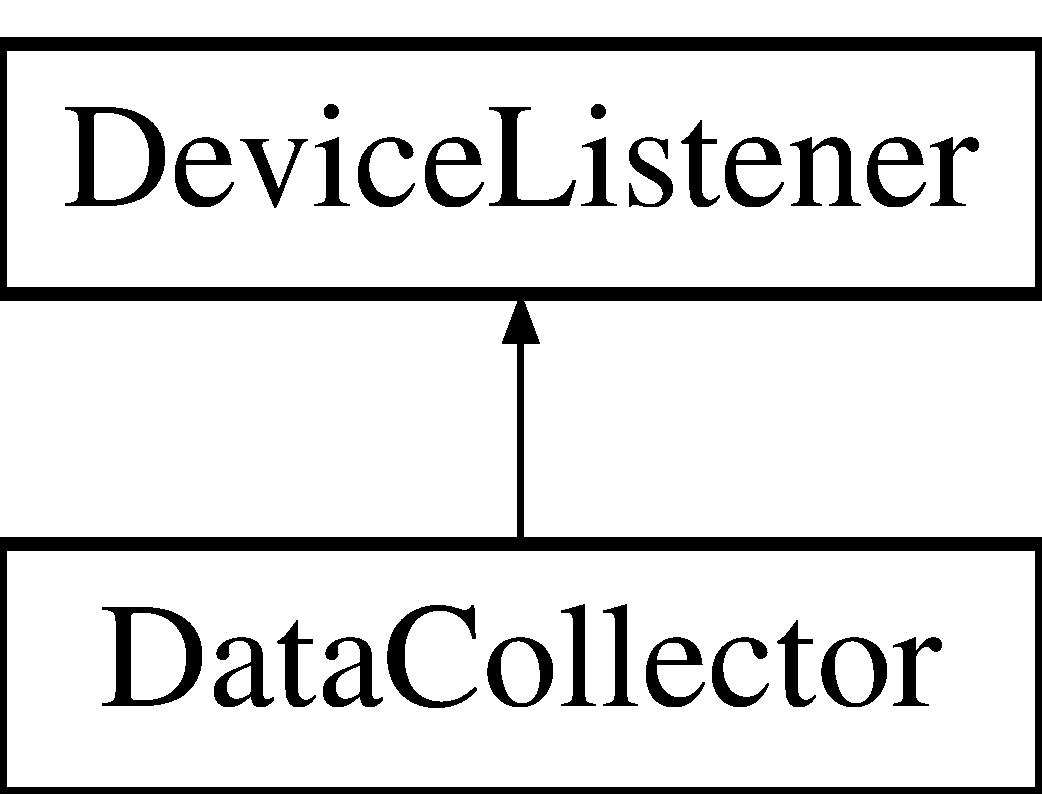
\includegraphics[height=2.000000cm]{class_data_collector}
\end{center}
\end{figure}
\subsection*{Public Member Functions}
\begin{DoxyCompactItemize}
\item 
\textbf{ Data\+Collector} ()
\item 
void \textbf{ on\+Orientation\+Data} (myo\+::\+Myo $\ast$myo, uint64\+\_\+t timestamp, const myo\+::\+Quaternion$<$ float $>$ \&rotation)
\item 
void \textbf{ on\+Accelerometer\+Data} (myo\+::\+Myo $\ast$myo, uint64\+\_\+t timestamp, const myo\+::\+Vector3$<$ float $>$ \&accel)
\item 
void \textbf{ on\+Gyroscope\+Data} (myo\+::\+Myo $\ast$myo, uint64\+\_\+t timestamp, const myo\+::\+Vector3$<$ float $>$ \&gyro)
\item 
void \textbf{ on\+Emg\+Data} (myo\+::\+Myo $\ast$myo, uint64\+\_\+t timestamp, const int8\+\_\+t $\ast$emg)
\item 
void \textbf{ on\+Battery\+Level\+Received} (myo\+::\+Myo $\ast$myo, uint64\+\_\+t timestamp, uint8\+\_\+t level)
\item 
void \textbf{ on\+Rssi} (myo\+::\+Myo $\ast$myo, uint64\+\_\+t timestamp, int8\+\_\+t rssi)
\item 
void \textbf{ on\+Connect} (myo\+::\+Myo $\ast$myo, uint64\+\_\+t timestamp, myo\+::\+Firmware\+Version firmware\+Version)
\item 
void \textbf{ on\+Disconnect} (myo\+::\+Myo $\ast$myo, uint64\+\_\+t timestamp)
\item 
myo\+::\+Quaternion$<$ float $>$ \textbf{ get\+Rotation} ()
\begin{DoxyCompactList}\small\item\em Gets rotation values. (updates automatically if class is conneced to myo\+::\+Hub) \end{DoxyCompactList}\item 
myo\+::\+Vector3$<$ float $>$ \textbf{ get\+Gyroscope} ()
\begin{DoxyCompactList}\small\item\em Gets the Gyroscope values. (updates automatically if class is conneced to myo\+::\+Hub) \end{DoxyCompactList}\item 
myo\+::\+Vector3$<$ float $>$ \textbf{ get\+Accelerometer} ()
\begin{DoxyCompactList}\small\item\em Gets all 8 E\+MG sensor Values. (updates automatically if class is conneced to myo\+::\+Hub) \end{DoxyCompactList}\item 
void \textbf{ get\+E\+MG} (std\+::array$<$ int8\+\_\+t, 8 $>$ $\ast$data)
\begin{DoxyCompactList}\small\item\em Gets all 8 E\+MG sensor Values. (updates automatically if class is conneced to myo\+::\+Hub) \end{DoxyCompactList}\item 
float \textbf{ get\+Rotation\+\_\+roll} ()
\begin{DoxyCompactList}\small\item\em Calculated Roll from rotation data. \end{DoxyCompactList}\item 
float \textbf{ get\+Rotation\+\_\+pitch} ()
\begin{DoxyCompactList}\small\item\em Calculated pitch from rotation data. \end{DoxyCompactList}\item 
float \textbf{ get\+Rotation\+\_\+yaw} ()
\begin{DoxyCompactList}\small\item\em Calculated yaw from rotation data. \end{DoxyCompactList}\item 
uint8\+\_\+t \textbf{ get\+Battery\+Level} ()
\begin{DoxyCompactList}\small\item\em Battery\+: This value wont update periodically. update via M\+Y\+O\+::request\+Battery\+Level() \end{DoxyCompactList}\item 
int8\+\_\+t \textbf{ get\+Bluetooth\+Range} ()
\begin{DoxyCompactList}\small\item\em Bluetooth\+: This value wont update periodically. update via update via M\+Y\+O\+::request\+Rssi();. \end{DoxyCompactList}\item 
bool \textbf{ get\+Connection\+Status} ()
\begin{DoxyCompactList}\small\item\em This value is automaticly updated. \end{DoxyCompactList}\end{DoxyCompactItemize}


\subsection{Detailed Description}
Contains all device information about a Myo Bracelet. 

It inherits all save data functions from myo\+::\+Device\+Listener, so to initalise the class from recieving data you have to put this line afer Myo initialisation\+: myo\+::hub.\+add\+Listener(\&datacollector); \begin{DoxyAuthor}{Author}
Ryan Vrosch 
\end{DoxyAuthor}
\begin{DoxyVersion}{Version}
1.\+1 
\end{DoxyVersion}
\begin{DoxyDate}{Date}
2018-\/11-\/30 
\end{DoxyDate}
\begin{DoxyWarning}{Warning}
Some params dont update themselves, and need to be called via myo\+::\+Myo. 
\end{DoxyWarning}
\begin{DoxyCopyright}{Copyright}
G\+NU Public License. 
\end{DoxyCopyright}


\subsection{Constructor \& Destructor Documentation}
\mbox{\label{class_data_collector_a6f7eccfdf026a83317c386a18d16397d}} 
\index{Data\+Collector@{Data\+Collector}!Data\+Collector@{Data\+Collector}}
\index{Data\+Collector@{Data\+Collector}!Data\+Collector@{Data\+Collector}}
\subsubsection{Data\+Collector()}
{\footnotesize\ttfamily Data\+Collector\+::\+Data\+Collector (\begin{DoxyParamCaption}{ }\end{DoxyParamCaption})}



\subsection{Member Function Documentation}
\mbox{\label{class_data_collector_a1ef7a2beb37a42d4ac887fef90ac8947}} 
\index{Data\+Collector@{Data\+Collector}!get\+Accelerometer@{get\+Accelerometer}}
\index{get\+Accelerometer@{get\+Accelerometer}!Data\+Collector@{Data\+Collector}}
\subsubsection{get\+Accelerometer()}
{\footnotesize\ttfamily myo\+::\+Vector3$<$float$>$ Data\+Collector\+::get\+Accelerometer (\begin{DoxyParamCaption}{ }\end{DoxyParamCaption})\hspace{0.3cm}{\ttfamily [inline]}}



Gets all 8 E\+MG sensor Values. (updates automatically if class is conneced to myo\+::\+Hub) 

\begin{DoxyReturn}{Returns}
accel myo\+::\+Vector3$<$float$>$ use raw value \+: .x() .y() .z(). 
\end{DoxyReturn}
\mbox{\label{class_data_collector_a376b4be3194c56e25084df4097968a46}} 
\index{Data\+Collector@{Data\+Collector}!get\+Battery\+Level@{get\+Battery\+Level}}
\index{get\+Battery\+Level@{get\+Battery\+Level}!Data\+Collector@{Data\+Collector}}
\subsubsection{get\+Battery\+Level()}
{\footnotesize\ttfamily uint8\+\_\+t Data\+Collector\+::get\+Battery\+Level (\begin{DoxyParamCaption}{ }\end{DoxyParamCaption})\hspace{0.3cm}{\ttfamily [inline]}}



Battery\+: This value wont update periodically. update via M\+Y\+O\+::request\+Battery\+Level() 

\begin{DoxyReturn}{Returns}
Battery Level in procentage. 
\end{DoxyReturn}
\mbox{\label{class_data_collector_a4992b2e777defed813c7ce15a73bc84b}} 
\index{Data\+Collector@{Data\+Collector}!get\+Bluetooth\+Range@{get\+Bluetooth\+Range}}
\index{get\+Bluetooth\+Range@{get\+Bluetooth\+Range}!Data\+Collector@{Data\+Collector}}
\subsubsection{get\+Bluetooth\+Range()}
{\footnotesize\ttfamily int8\+\_\+t Data\+Collector\+::get\+Bluetooth\+Range (\begin{DoxyParamCaption}{ }\end{DoxyParamCaption})\hspace{0.3cm}{\ttfamily [inline]}}



Bluetooth\+: This value wont update periodically. update via update via M\+Y\+O\+::request\+Rssi();. 

\begin{DoxyReturn}{Returns}
bluetooth range 0-\/127. 
\end{DoxyReturn}
\mbox{\label{class_data_collector_a2dbac95176fb77c1714573e41ba4490f}} 
\index{Data\+Collector@{Data\+Collector}!get\+Connection\+Status@{get\+Connection\+Status}}
\index{get\+Connection\+Status@{get\+Connection\+Status}!Data\+Collector@{Data\+Collector}}
\subsubsection{get\+Connection\+Status()}
{\footnotesize\ttfamily bool Data\+Collector\+::get\+Connection\+Status (\begin{DoxyParamCaption}{ }\end{DoxyParamCaption})\hspace{0.3cm}{\ttfamily [inline]}}



This value is automaticly updated. 

\begin{DoxyReturn}{Returns}
connection status (bool) true = Connected $\vert$ false = disconnected. 
\end{DoxyReturn}
\mbox{\label{class_data_collector_a6994bc51d1e7cbcaeca954a4ba7f8103}} 
\index{Data\+Collector@{Data\+Collector}!get\+E\+MG@{get\+E\+MG}}
\index{get\+E\+MG@{get\+E\+MG}!Data\+Collector@{Data\+Collector}}
\subsubsection{get\+E\+M\+G()}
{\footnotesize\ttfamily void Data\+Collector\+::get\+E\+MG (\begin{DoxyParamCaption}\item[{std\+::array$<$ int8\+\_\+t, 8 $>$ $\ast$}]{data }\end{DoxyParamCaption})\hspace{0.3cm}{\ttfamily [inline]}}



Gets all 8 E\+MG sensor Values. (updates automatically if class is conneced to myo\+::\+Hub) 


\begin{DoxyParams}[1]{Parameters}
\mbox{\tt in,out}  & {\em data} & returns emg data if $\ast$data != null. \\
\hline
\end{DoxyParams}
\mbox{\label{class_data_collector_a04ad19d96b8574ff7c9f945cd1c5ddc6}} 
\index{Data\+Collector@{Data\+Collector}!get\+Gyroscope@{get\+Gyroscope}}
\index{get\+Gyroscope@{get\+Gyroscope}!Data\+Collector@{Data\+Collector}}
\subsubsection{get\+Gyroscope()}
{\footnotesize\ttfamily myo\+::\+Vector3$<$float$>$ Data\+Collector\+::get\+Gyroscope (\begin{DoxyParamCaption}{ }\end{DoxyParamCaption})\hspace{0.3cm}{\ttfamily [inline]}}



Gets the Gyroscope values. (updates automatically if class is conneced to myo\+::\+Hub) 

\begin{DoxyReturn}{Returns}
accel myo\+::\+Vector3$<$float$>$ use raw value \+: .x() .y() .z(). 
\end{DoxyReturn}
\mbox{\label{class_data_collector_a46a7e8adb8679fde1021fe89ed0d0be0}} 
\index{Data\+Collector@{Data\+Collector}!get\+Rotation@{get\+Rotation}}
\index{get\+Rotation@{get\+Rotation}!Data\+Collector@{Data\+Collector}}
\subsubsection{get\+Rotation()}
{\footnotesize\ttfamily myo\+::\+Quaternion$<$float$>$ Data\+Collector\+::get\+Rotation (\begin{DoxyParamCaption}{ }\end{DoxyParamCaption})\hspace{0.3cm}{\ttfamily [inline]}}



Gets rotation values. (updates automatically if class is conneced to myo\+::\+Hub) 

\begin{DoxyReturn}{Returns}
myo\+::\+Quaternion$<$float$>$ use raw value\+: .x() .y() .z() .w(). 
\end{DoxyReturn}
\mbox{\label{class_data_collector_a603dbbfb9d59838c775f51e1e695e638}} 
\index{Data\+Collector@{Data\+Collector}!get\+Rotation\+\_\+pitch@{get\+Rotation\+\_\+pitch}}
\index{get\+Rotation\+\_\+pitch@{get\+Rotation\+\_\+pitch}!Data\+Collector@{Data\+Collector}}
\subsubsection{get\+Rotation\+\_\+pitch()}
{\footnotesize\ttfamily float Data\+Collector\+::get\+Rotation\+\_\+pitch (\begin{DoxyParamCaption}{ }\end{DoxyParamCaption})\hspace{0.3cm}{\ttfamily [inline]}}



Calculated pitch from rotation data. 

\begin{DoxyReturn}{Returns}
Pitch in radial. 
\end{DoxyReturn}
\mbox{\label{class_data_collector_a4e761ba292f93b5ac18e05a860a697ab}} 
\index{Data\+Collector@{Data\+Collector}!get\+Rotation\+\_\+roll@{get\+Rotation\+\_\+roll}}
\index{get\+Rotation\+\_\+roll@{get\+Rotation\+\_\+roll}!Data\+Collector@{Data\+Collector}}
\subsubsection{get\+Rotation\+\_\+roll()}
{\footnotesize\ttfamily float Data\+Collector\+::get\+Rotation\+\_\+roll (\begin{DoxyParamCaption}{ }\end{DoxyParamCaption})\hspace{0.3cm}{\ttfamily [inline]}}



Calculated Roll from rotation data. 

\begin{DoxyReturn}{Returns}
Roll in radial. 
\end{DoxyReturn}
\mbox{\label{class_data_collector_a45175c5352dd3870c2d1cf99c4b2d938}} 
\index{Data\+Collector@{Data\+Collector}!get\+Rotation\+\_\+yaw@{get\+Rotation\+\_\+yaw}}
\index{get\+Rotation\+\_\+yaw@{get\+Rotation\+\_\+yaw}!Data\+Collector@{Data\+Collector}}
\subsubsection{get\+Rotation\+\_\+yaw()}
{\footnotesize\ttfamily float Data\+Collector\+::get\+Rotation\+\_\+yaw (\begin{DoxyParamCaption}{ }\end{DoxyParamCaption})\hspace{0.3cm}{\ttfamily [inline]}}



Calculated yaw from rotation data. 

\begin{DoxyReturn}{Returns}
Yaw in radial. 
\end{DoxyReturn}
\mbox{\label{class_data_collector_af284c1bda701eb04d8278848672a1be6}} 
\index{Data\+Collector@{Data\+Collector}!on\+Accelerometer\+Data@{on\+Accelerometer\+Data}}
\index{on\+Accelerometer\+Data@{on\+Accelerometer\+Data}!Data\+Collector@{Data\+Collector}}
\subsubsection{on\+Accelerometer\+Data()}
{\footnotesize\ttfamily void Data\+Collector\+::on\+Accelerometer\+Data (\begin{DoxyParamCaption}\item[{myo\+::\+Myo $\ast$}]{myo,  }\item[{uint64\+\_\+t}]{timestamp,  }\item[{const myo\+::\+Vector3$<$ float $>$ \&}]{accel }\end{DoxyParamCaption})}

\mbox{\label{class_data_collector_a56a6c61925d54439459fc1599f76c601}} 
\index{Data\+Collector@{Data\+Collector}!on\+Battery\+Level\+Received@{on\+Battery\+Level\+Received}}
\index{on\+Battery\+Level\+Received@{on\+Battery\+Level\+Received}!Data\+Collector@{Data\+Collector}}
\subsubsection{on\+Battery\+Level\+Received()}
{\footnotesize\ttfamily void Data\+Collector\+::on\+Battery\+Level\+Received (\begin{DoxyParamCaption}\item[{myo\+::\+Myo $\ast$}]{myo,  }\item[{uint64\+\_\+t}]{timestamp,  }\item[{uint8\+\_\+t}]{level }\end{DoxyParamCaption})}

\mbox{\label{class_data_collector_a8e6ee72005537474eb45f2a9310fa540}} 
\index{Data\+Collector@{Data\+Collector}!on\+Connect@{on\+Connect}}
\index{on\+Connect@{on\+Connect}!Data\+Collector@{Data\+Collector}}
\subsubsection{on\+Connect()}
{\footnotesize\ttfamily void Data\+Collector\+::on\+Connect (\begin{DoxyParamCaption}\item[{myo\+::\+Myo $\ast$}]{myo,  }\item[{uint64\+\_\+t}]{timestamp,  }\item[{myo\+::\+Firmware\+Version}]{firmware\+Version }\end{DoxyParamCaption})}

\mbox{\label{class_data_collector_a89d1d780cdf635c607707f90b0665d50}} 
\index{Data\+Collector@{Data\+Collector}!on\+Disconnect@{on\+Disconnect}}
\index{on\+Disconnect@{on\+Disconnect}!Data\+Collector@{Data\+Collector}}
\subsubsection{on\+Disconnect()}
{\footnotesize\ttfamily void Data\+Collector\+::on\+Disconnect (\begin{DoxyParamCaption}\item[{myo\+::\+Myo $\ast$}]{myo,  }\item[{uint64\+\_\+t}]{timestamp }\end{DoxyParamCaption})}

\mbox{\label{class_data_collector_a43639de09ccb9c540a3d21d267e7460a}} 
\index{Data\+Collector@{Data\+Collector}!on\+Emg\+Data@{on\+Emg\+Data}}
\index{on\+Emg\+Data@{on\+Emg\+Data}!Data\+Collector@{Data\+Collector}}
\subsubsection{on\+Emg\+Data()}
{\footnotesize\ttfamily void Data\+Collector\+::on\+Emg\+Data (\begin{DoxyParamCaption}\item[{myo\+::\+Myo $\ast$}]{myo,  }\item[{uint64\+\_\+t}]{timestamp,  }\item[{const int8\+\_\+t $\ast$}]{emg }\end{DoxyParamCaption})}

\mbox{\label{class_data_collector_a46ee5fda02554a8d84a0f449026dcfac}} 
\index{Data\+Collector@{Data\+Collector}!on\+Gyroscope\+Data@{on\+Gyroscope\+Data}}
\index{on\+Gyroscope\+Data@{on\+Gyroscope\+Data}!Data\+Collector@{Data\+Collector}}
\subsubsection{on\+Gyroscope\+Data()}
{\footnotesize\ttfamily void Data\+Collector\+::on\+Gyroscope\+Data (\begin{DoxyParamCaption}\item[{myo\+::\+Myo $\ast$}]{myo,  }\item[{uint64\+\_\+t}]{timestamp,  }\item[{const myo\+::\+Vector3$<$ float $>$ \&}]{gyro }\end{DoxyParamCaption})}

\mbox{\label{class_data_collector_a7e54df882eed064e4059b3361dff796f}} 
\index{Data\+Collector@{Data\+Collector}!on\+Orientation\+Data@{on\+Orientation\+Data}}
\index{on\+Orientation\+Data@{on\+Orientation\+Data}!Data\+Collector@{Data\+Collector}}
\subsubsection{on\+Orientation\+Data()}
{\footnotesize\ttfamily void Data\+Collector\+::on\+Orientation\+Data (\begin{DoxyParamCaption}\item[{myo\+::\+Myo $\ast$}]{myo,  }\item[{uint64\+\_\+t}]{timestamp,  }\item[{const myo\+::\+Quaternion$<$ float $>$ \&}]{rotation }\end{DoxyParamCaption})}

\mbox{\label{class_data_collector_aff0d95e10b014c460bf859abd6a01f74}} 
\index{Data\+Collector@{Data\+Collector}!on\+Rssi@{on\+Rssi}}
\index{on\+Rssi@{on\+Rssi}!Data\+Collector@{Data\+Collector}}
\subsubsection{on\+Rssi()}
{\footnotesize\ttfamily void Data\+Collector\+::on\+Rssi (\begin{DoxyParamCaption}\item[{myo\+::\+Myo $\ast$}]{myo,  }\item[{uint64\+\_\+t}]{timestamp,  }\item[{int8\+\_\+t}]{rssi }\end{DoxyParamCaption})}



The documentation for this class was generated from the following files\+:\begin{DoxyCompactItemize}
\item 
\textbf{ Data\+Collector.\+h}\item 
\textbf{ Data\+Collector.\+cpp}\end{DoxyCompactItemize}

\section{Peak\+Detector$<$ T $>$ Class Template Reference}
\label{class_peak_detector}\index{Peak\+Detector$<$ T $>$@{Peak\+Detector$<$ T $>$}}


Detects peaks in realtime signals by calculating the direction of a signal.  




{\ttfamily \#include $<$Peak\+Detector.\+h$>$}

\subsection*{Public Member Functions}
\begin{DoxyCompactItemize}
\item 
\textbf{ Peak\+Detector} (int measure\+Length, T minimum\+Sample\+Difference, T minimum\+Peak\+Threshold, T mimimum\+Peak\+Offset)
\begin{DoxyCompactList}\small\item\em initialises all sample settings. \end{DoxyCompactList}\item 
\textbf{ $\sim$\+Peak\+Detector} ()
\item 
void \textbf{ Calculate} (T Sample)
\begin{DoxyCompactList}\small\item\em Calculates the signal if a direction is detected. use \doxyref{Get\+Peak()}{p.}{class_peak_detector_a72f7916aa1d26388c9d70eee1cd5e3bc} to see if a peak is detected. \end{DoxyCompactList}\item 
\textbf{ Peak\+Type} \textbf{ Get\+Peak} ()
\begin{DoxyCompactList}\small\item\em Call \doxyref{Calculate(\+T sample)}{p.}{class_peak_detector_a888b9d29612caf03e7417ab3593f6392} before Getting the peakvalue. \end{DoxyCompactList}\item 
T \textbf{ Get\+Raw\+Peek\+Value} ()
\begin{DoxyCompactList}\small\item\em Call \doxyref{Calculate(\+T sample)}{p.}{class_peak_detector_a888b9d29612caf03e7417ab3593f6392} before Getting the Raw\+Peek\+Value. \end{DoxyCompactList}\end{DoxyCompactItemize}


\subsection{Detailed Description}
\subsubsection*{template$<$class T$>$\newline
class Peak\+Detector$<$ T $>$}

Detects peaks in realtime signals by calculating the direction of a signal. 

\begin{DoxyAuthor}{Author}
Ryan Vrosch \& Tim Hoenselaar 
\end{DoxyAuthor}
\begin{DoxyVersion}{Version}
1.\+3 
\end{DoxyVersion}
\begin{DoxyDate}{Date}
2018-\/11-\/30 
\end{DoxyDate}
\begin{DoxyCopyright}{Copyright}
G\+NU Public License. 
\end{DoxyCopyright}


\subsection{Constructor \& Destructor Documentation}
\mbox{\label{class_peak_detector_a616829654acf46b8574903d9abcdaf9d}} 
\index{Peak\+Detector@{Peak\+Detector}!Peak\+Detector@{Peak\+Detector}}
\index{Peak\+Detector@{Peak\+Detector}!Peak\+Detector@{Peak\+Detector}}
\subsubsection{Peak\+Detector()}
{\footnotesize\ttfamily template$<$class T $>$ \\
\textbf{ Peak\+Detector}$<$ T $>$\+::\textbf{ Peak\+Detector} (\begin{DoxyParamCaption}\item[{int}]{measure\+Length,  }\item[{T}]{minimum\+Sample\+Difference,  }\item[{T}]{minimum\+Peak\+Threshold,  }\item[{T}]{mimimum\+Peak\+Offset }\end{DoxyParamCaption})}



initialises all sample settings. 


\begin{DoxyParams}{Parameters}
{\em measure\+Length} & Length of the sampling array, has to be an even number. \\
\hline
{\em minimum\+Sample\+Difference} & If The sample is lower then previous sample\+Difference the sample is discarded. \\
\hline
{\em minimum\+Peak\+Threshold} & Minimum Threshold relative to Peakoffset. If Sample is lower than Peakthreshold no peak will be detected. this value is the same for positive and negative samples. \\
\hline
{\em mimimum\+Peak\+Offset} & Sets the baseline of the peakthreshold. \\
\hline
\end{DoxyParams}
\mbox{\label{class_peak_detector_a950c3287299cf1352cb7c32de2f54384}} 
\index{Peak\+Detector@{Peak\+Detector}!````~Peak\+Detector@{$\sim$\+Peak\+Detector}}
\index{````~Peak\+Detector@{$\sim$\+Peak\+Detector}!Peak\+Detector@{Peak\+Detector}}
\subsubsection{$\sim$\+Peak\+Detector()}
{\footnotesize\ttfamily template$<$class T $>$ \\
\textbf{ Peak\+Detector}$<$ T $>$\+::$\sim$\textbf{ Peak\+Detector} (\begin{DoxyParamCaption}{ }\end{DoxyParamCaption})}



\subsection{Member Function Documentation}
\mbox{\label{class_peak_detector_a888b9d29612caf03e7417ab3593f6392}} 
\index{Peak\+Detector@{Peak\+Detector}!Calculate@{Calculate}}
\index{Calculate@{Calculate}!Peak\+Detector@{Peak\+Detector}}
\subsubsection{Calculate()}
{\footnotesize\ttfamily template$<$class T $>$ \\
void \textbf{ Peak\+Detector}$<$ T $>$\+::Calculate (\begin{DoxyParamCaption}\item[{T}]{sample }\end{DoxyParamCaption})}



Calculates the signal if a direction is detected. use \doxyref{Get\+Peak()}{p.}{class_peak_detector_a72f7916aa1d26388c9d70eee1cd5e3bc} to see if a peak is detected. 


\begin{DoxyParams}{Parameters}
{\em sample} & signal to calculate \\
\hline
\end{DoxyParams}
\mbox{\label{class_peak_detector_a72f7916aa1d26388c9d70eee1cd5e3bc}} 
\index{Peak\+Detector@{Peak\+Detector}!Get\+Peak@{Get\+Peak}}
\index{Get\+Peak@{Get\+Peak}!Peak\+Detector@{Peak\+Detector}}
\subsubsection{Get\+Peak()}
{\footnotesize\ttfamily template$<$class T $>$ \\
\textbf{ Peak\+Type} \textbf{ Peak\+Detector}$<$ T $>$\+::Get\+Peak (\begin{DoxyParamCaption}{ }\end{DoxyParamCaption})}



Call \doxyref{Calculate(\+T sample)}{p.}{class_peak_detector_a888b9d29612caf03e7417ab3593f6392} before Getting the peakvalue. 

\mbox{\label{class_peak_detector_aebfc5583c4c696119bbe834b1474d896}} 
\index{Peak\+Detector@{Peak\+Detector}!Get\+Raw\+Peek\+Value@{Get\+Raw\+Peek\+Value}}
\index{Get\+Raw\+Peek\+Value@{Get\+Raw\+Peek\+Value}!Peak\+Detector@{Peak\+Detector}}
\subsubsection{Get\+Raw\+Peek\+Value()}
{\footnotesize\ttfamily template$<$class T $>$ \\
T \textbf{ Peak\+Detector}$<$ T $>$\+::Get\+Raw\+Peek\+Value (\begin{DoxyParamCaption}{ }\end{DoxyParamCaption})}



Call \doxyref{Calculate(\+T sample)}{p.}{class_peak_detector_a888b9d29612caf03e7417ab3593f6392} before Getting the Raw\+Peek\+Value. 



The documentation for this class was generated from the following files\+:\begin{DoxyCompactItemize}
\item 
\textbf{ Peak\+Detector.\+h}\item 
\textbf{ Peak\+Detector.\+cpp}\end{DoxyCompactItemize}

\input{class_u_d_p_client}
\chapter{File Documentation}
\section{Communicator.\+cpp File Reference}
\label{_communicator_8cpp}\index{Communicator.\+cpp@{Communicator.\+cpp}}
{\ttfamily \#include \char`\"{}Communicator.\+h\char`\"{}}\newline

\section{Communicator.\+h File Reference}
\label{_communicator_8h}\index{Communicator.\+h@{Communicator.\+h}}
{\ttfamily \#include $<$Windows.\+h$>$}\newline
{\ttfamily \#include $<$tchar.\+h$>$}\newline
{\ttfamily \#include $<$stdio.\+h$>$}\newline
{\ttfamily \#include $<$string$>$}\newline
{\ttfamily \#include $<$exception$>$}\newline
\subsection*{Classes}
\begin{DoxyCompactItemize}
\item 
class \textbf{ Communicator}
\end{DoxyCompactItemize}

\hypertarget{_data_collector_8cpp}{}\section{Data\+Collector.\+cpp File Reference}
\label{_data_collector_8cpp}\index{Data\+Collector.\+cpp@{Data\+Collector.\+cpp}}
{\ttfamily \#include \char`\"{}Data\+Collector.\+h\char`\"{}}\newline
{\ttfamily \#include $<$cmath$>$}\newline

\hypertarget{_data_collector_8h}{}\section{Data\+Collector.\+h File Reference}
\label{_data_collector_8h}\index{Data\+Collector.\+h@{Data\+Collector.\+h}}
{\ttfamily \#include $<$myo/myo.\+hpp$>$}\newline
{\ttfamily \#include $<$array$>$}\newline
\subsection*{Classes}
\begin{DoxyCompactItemize}
\item 
class \mbox{\hyperlink{class_data_collector}{Data\+Collector}}
\begin{DoxyCompactList}\small\item\em Contains all device information about a Myo Bracelet. \end{DoxyCompactList}\end{DoxyCompactItemize}

\section{Myo.\+cpp File Reference}
\label{_myo_8cpp}\index{Myo.\+cpp@{Myo.\+cpp}}
{\ttfamily \#include $<$iostream$>$}\newline
{\ttfamily \#include $<$iomanip$>$}\newline
{\ttfamily \#include $<$stdexcept$>$}\newline
{\ttfamily \#include $<$string$>$}\newline
{\ttfamily \#include $<$string.\+h$>$}\newline
{\ttfamily \#include $<$fstream$>$}\newline
{\ttfamily \#include $<$myo/myo.\+hpp$>$}\newline
{\ttfamily \#include \char`\"{}Data\+Collector.\+h\char`\"{}}\newline
{\ttfamily \#include \char`\"{}Communicator.\+h\char`\"{}}\newline
{\ttfamily \#include \char`\"{}Peak\+Detector.\+h\char`\"{}}\newline
\subsection*{Macros}
\begin{DoxyCompactItemize}
\item 
\#define \textbf{ \+\_\+\+U\+S\+E\+\_\+\+M\+A\+T\+H\+\_\+\+D\+E\+F\+I\+N\+ES}
\end{DoxyCompactItemize}
\subsection*{Functions}
\begin{DoxyCompactItemize}
\item 
int \textbf{ main} (int argc, char $\ast$$\ast$argv)
\end{DoxyCompactItemize}
\subsection*{Variables}
\begin{DoxyCompactItemize}
\item 
constexpr auto \textbf{ Connected} = true
\item 
const char \textbf{ filename} [$\,$] = \char`\"{}test.\+txt \char`\"{}
\end{DoxyCompactItemize}


\subsection{Macro Definition Documentation}
\mbox{\label{_myo_8cpp_a525335710b53cb064ca56b936120431e}} 
\index{Myo.\+cpp@{Myo.\+cpp}!\+\_\+\+U\+S\+E\+\_\+\+M\+A\+T\+H\+\_\+\+D\+E\+F\+I\+N\+ES@{\+\_\+\+U\+S\+E\+\_\+\+M\+A\+T\+H\+\_\+\+D\+E\+F\+I\+N\+ES}}
\index{\+\_\+\+U\+S\+E\+\_\+\+M\+A\+T\+H\+\_\+\+D\+E\+F\+I\+N\+ES@{\+\_\+\+U\+S\+E\+\_\+\+M\+A\+T\+H\+\_\+\+D\+E\+F\+I\+N\+ES}!Myo.\+cpp@{Myo.\+cpp}}
\subsubsection{\+\_\+\+U\+S\+E\+\_\+\+M\+A\+T\+H\+\_\+\+D\+E\+F\+I\+N\+ES}
{\footnotesize\ttfamily \#define \+\_\+\+U\+S\+E\+\_\+\+M\+A\+T\+H\+\_\+\+D\+E\+F\+I\+N\+ES}



\subsection{Function Documentation}
\mbox{\label{_myo_8cpp_a3c04138a5bfe5d72780bb7e82a18e627}} 
\index{Myo.\+cpp@{Myo.\+cpp}!main@{main}}
\index{main@{main}!Myo.\+cpp@{Myo.\+cpp}}
\subsubsection{main()}
{\footnotesize\ttfamily int main (\begin{DoxyParamCaption}\item[{int}]{argc,  }\item[{char $\ast$$\ast$}]{argv }\end{DoxyParamCaption})}



\subsection{Variable Documentation}
\mbox{\label{_myo_8cpp_afd1c6f44ddce5cb060370262eecd9c17}} 
\index{Myo.\+cpp@{Myo.\+cpp}!Connected@{Connected}}
\index{Connected@{Connected}!Myo.\+cpp@{Myo.\+cpp}}
\subsubsection{Connected}
{\footnotesize\ttfamily constexpr auto Connected = true}

\mbox{\label{_myo_8cpp_a1dd0092466ef147d6873cd10f5d5e38b}} 
\index{Myo.\+cpp@{Myo.\+cpp}!filename@{filename}}
\index{filename@{filename}!Myo.\+cpp@{Myo.\+cpp}}
\subsubsection{filename}
{\footnotesize\ttfamily const char filename[$\,$] = \char`\"{}test.\+txt \char`\"{}}


\input{pch_8cpp}
\input{pch_8h}
\hypertarget{_peak_detector_8cpp}{}\section{Peak\+Detector.\+cpp File Reference}
\label{_peak_detector_8cpp}\index{Peak\+Detector.\+cpp@{Peak\+Detector.\+cpp}}
{\ttfamily \#include \char`\"{}Peak\+Detector.\+h\char`\"{}}\newline
{\ttfamily \#include $<$algorithm$>$}\newline
{\ttfamily \#include $<$vector$>$}\newline

\hypertarget{_peak_detector_8h}{}\section{Peak\+Detector.\+h File Reference}
\label{_peak_detector_8h}\index{Peak\+Detector.\+h@{Peak\+Detector.\+h}}
{\ttfamily \#include $<$vector$>$}\newline
\subsection*{Classes}
\begin{DoxyCompactItemize}
\item 
class \mbox{\hyperlink{class_peak_detector}{Peak\+Detector$<$ T $>$}}
\end{DoxyCompactItemize}
\subsection*{Enumerations}
\begin{DoxyCompactItemize}
\item 
enum \mbox{\hyperlink{_peak_detector_8h_a4791e14c9f62a95fdf58cd8b41ca6a08}{Peak\+Type}} \+: uint8\+\_\+t \{ \mbox{\hyperlink{_peak_detector_8h_a4791e14c9f62a95fdf58cd8b41ca6a08af3e33603bf389e5b337ee5bdbc9558b9}{positive}}, 
\mbox{\hyperlink{_peak_detector_8h_a4791e14c9f62a95fdf58cd8b41ca6a08a7b1174d620ccd8d2a049d8440aa1fc4d}{negative}}, 
\mbox{\hyperlink{_peak_detector_8h_a4791e14c9f62a95fdf58cd8b41ca6a08aae7ff4c6474ee46308f274e0f7174bee}{none\+Detected}}
 \}
\end{DoxyCompactItemize}


\subsection{Enumeration Type Documentation}
\mbox{\Hypertarget{_peak_detector_8h_a4791e14c9f62a95fdf58cd8b41ca6a08}\label{_peak_detector_8h_a4791e14c9f62a95fdf58cd8b41ca6a08}} 
\index{Peak\+Detector.\+h@{Peak\+Detector.\+h}!Peak\+Type@{Peak\+Type}}
\index{Peak\+Type@{Peak\+Type}!Peak\+Detector.\+h@{Peak\+Detector.\+h}}
\subsubsection{\texorpdfstring{Peak\+Type}{PeakType}}
{\footnotesize\ttfamily enum \mbox{\hyperlink{_peak_detector_8h_a4791e14c9f62a95fdf58cd8b41ca6a08}{Peak\+Type}} \+: uint8\+\_\+t}

\begin{DoxyEnumFields}{Enumerator}
\raisebox{\heightof{T}}[0pt][0pt]{\index{positive@{positive}!Peak\+Detector.\+h@{Peak\+Detector.\+h}}\index{Peak\+Detector.\+h@{Peak\+Detector.\+h}!positive@{positive}}}\mbox{\Hypertarget{_peak_detector_8h_a4791e14c9f62a95fdf58cd8b41ca6a08af3e33603bf389e5b337ee5bdbc9558b9}\label{_peak_detector_8h_a4791e14c9f62a95fdf58cd8b41ca6a08af3e33603bf389e5b337ee5bdbc9558b9}} 
positive&\\
\hline

\raisebox{\heightof{T}}[0pt][0pt]{\index{negative@{negative}!Peak\+Detector.\+h@{Peak\+Detector.\+h}}\index{Peak\+Detector.\+h@{Peak\+Detector.\+h}!negative@{negative}}}\mbox{\Hypertarget{_peak_detector_8h_a4791e14c9f62a95fdf58cd8b41ca6a08a7b1174d620ccd8d2a049d8440aa1fc4d}\label{_peak_detector_8h_a4791e14c9f62a95fdf58cd8b41ca6a08a7b1174d620ccd8d2a049d8440aa1fc4d}} 
negative&\\
\hline

\raisebox{\heightof{T}}[0pt][0pt]{\index{none\+Detected@{none\+Detected}!Peak\+Detector.\+h@{Peak\+Detector.\+h}}\index{Peak\+Detector.\+h@{Peak\+Detector.\+h}!none\+Detected@{none\+Detected}}}\mbox{\Hypertarget{_peak_detector_8h_a4791e14c9f62a95fdf58cd8b41ca6a08aae7ff4c6474ee46308f274e0f7174bee}\label{_peak_detector_8h_a4791e14c9f62a95fdf58cd8b41ca6a08aae7ff4c6474ee46308f274e0f7174bee}} 
none\+Detected&\\
\hline

\end{DoxyEnumFields}


Definition at line 15 of file Peak\+Detector.\+h.


\input{_u_d_p_client_8cpp}
\input{_u_d_p_client_8h}
%--- End generated contents ---

% Index
\backmatter
\newpage
\phantomsection
\clearemptydoublepage
\addcontentsline{toc}{chapter}{Index}
\printindex

\end{document}
